\chapter{The Large Hadron Collider}
   The chapter on the Large Hadron Collider provides a bit of overview on the purpose and operation principle of the collider. It also provides the information on the special low pile-up run which is the main source of experimental data for the W boson transverse momentum measurement analysis.
   
   
    \section{Introduction} 
        The study of elementary particles naturally demands a stable source of particles. At the dawn of particle physics the two main sources were radioactive materials and cosmic rays. However soon researchers became in need of a more reliable source of particles in terms of particle energy, luminosity and experimental repeatability. This has commenced the era of particle accelerators.\\
        The first examples of particle accelerators were designed in the late 1920s and in the early 1930s. Two different designs emerged: linear and circular. The former accelerates particles via electric field during the single pass through the machine, while the latter uses magnetic field to make accelerated particles go in circles allowing to re-accelerate the same beam many times. On the other hand the circular design comprises energy losses due to Bremsstrahlung radiation.\\
        In the second half of the XX$^{th}$ century the accelerators gradually got bigger and bigger in both size and centre-of-mass energy of the accelerated particles. This has allowed to create an experimental basis for the development of modern particle physics, notably the Standard Model.\\
        Up to this day the biggest particle accelerator with the highest centre-of-mass energy is the Large Hadron Collider (LHC). The LHC is a circular collider that lies in a tunnel of 27 km under the French-Swiss border next to Geneva \cite{Bruning:2668521}. In 2012 the two biggest experiments of LHC have claimed the discovery of the Higgs boson, the last elementary particle predicted by the Standard Model which was not yet discovered by that time. \cite{higgs_atlas}, \cite{higgs_cms}.
        
        \section{The LHC running sequence}
                   \begin{figure}[htpb]
        	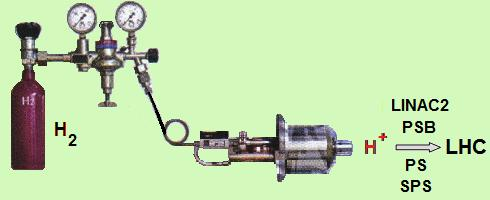
\includegraphics[width=\textwidth,keepaspectratio]{hydro_tank.jpg}
        	\caption{A hydrogen tank supplies LHC with protons \cite{hydro}.}
        	\label{fig::hydro}
        \end{figure}
        	
        It takes quite a journey for a proton to travel from a hydrogen tank (Fig. \ref{fig::hydro}) into one of the LHC's collision points. A resourceful system of pre-accelerators is necessary to make the proton beam ready to get injected into one of the two LHC beam pipes. The LHC accelerator complex was not built from scratch - it uses vast CERN infrastructure, that was built for the previous particle physics experiments. \\
        After stripping the electrons off the atoms of hydrogen using a magnetic field the yielded protons get accelerated to the energy of 50 MeV by the Linac 2\footnote{After Run 2 the Linac 2 has been decommissioned to be succeeded by Linac 4.} \cite{sequence}. After that the beam gets into the Proton Synchrotron Booster (PSB) to be accelerated to 1.4 GeV. The next link of the pre-acceleration chain is the Proton Synchrotron (PS) - a true veteran among CERN accelerators that first accelerated protons in 1959 breaking the world record in acceleration energy. Currently thanks to PSB and other modifications it can sustain proton beam intensity ~1000 times larger than back in 1959. The PS accelerates the beam up to 25 GeV and conveys it further to the Super Proton Synchrotron (SPS) - the second-largest particle accelerator at CERN. Back in 1983 the massive electroweak bosons were discovered at the SPS but even now it serves as a main accelerator for the NA61/SHINE, NA62 and COMPASS experiments. The SPS raises the beam energy to 450 GeV and finally injects it into the LHC beam pipes (see Fig \ref{fig::layout}).\\
   

	\begin{figure}[htbp]
	\begin{subfigure}[t]{0.48\textwidth}
		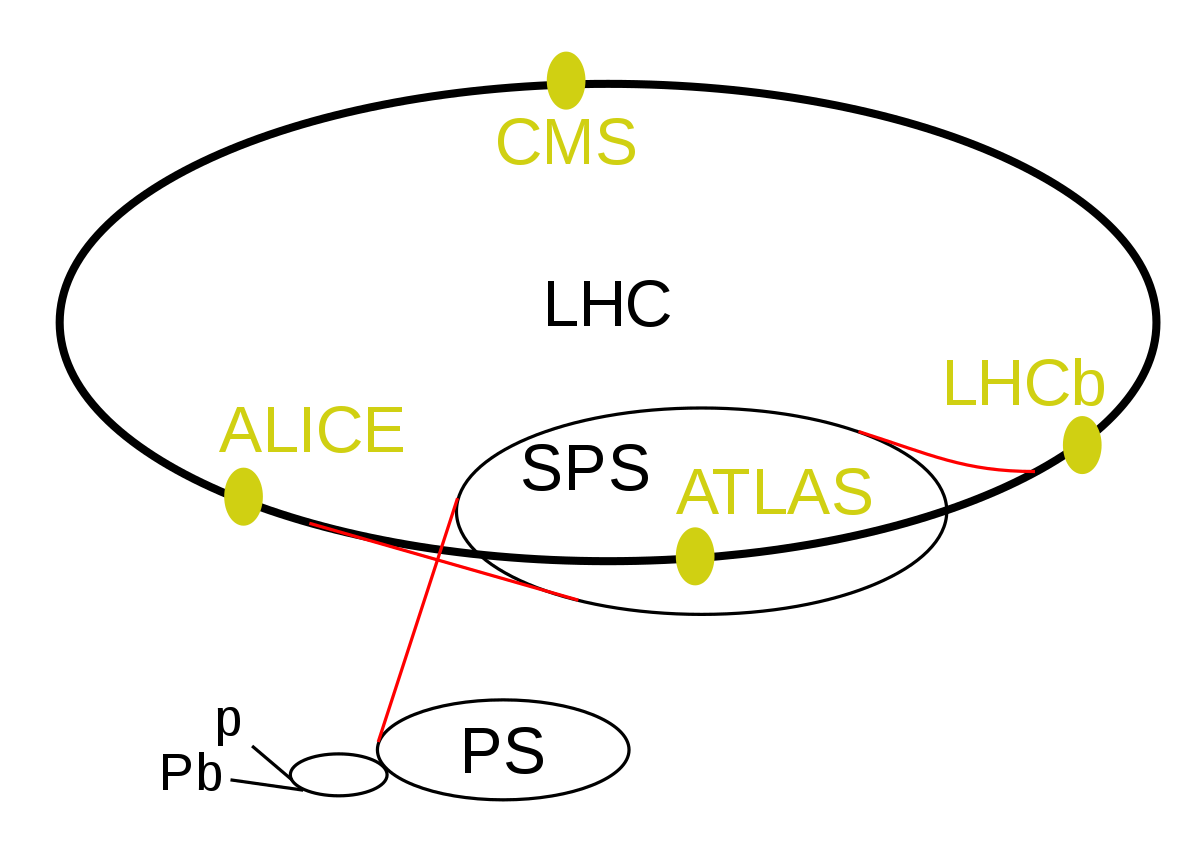
\includegraphics[width=\textwidth,keepaspectratio]{LHC.png}
		\caption[Acceleration sequence]{Acceleration sequence \cite{sequence}.}
		\label{fig::seq}
	\end{subfigure}
	\hfill
	\begin{subfigure}[t]{0.48\textwidth}
		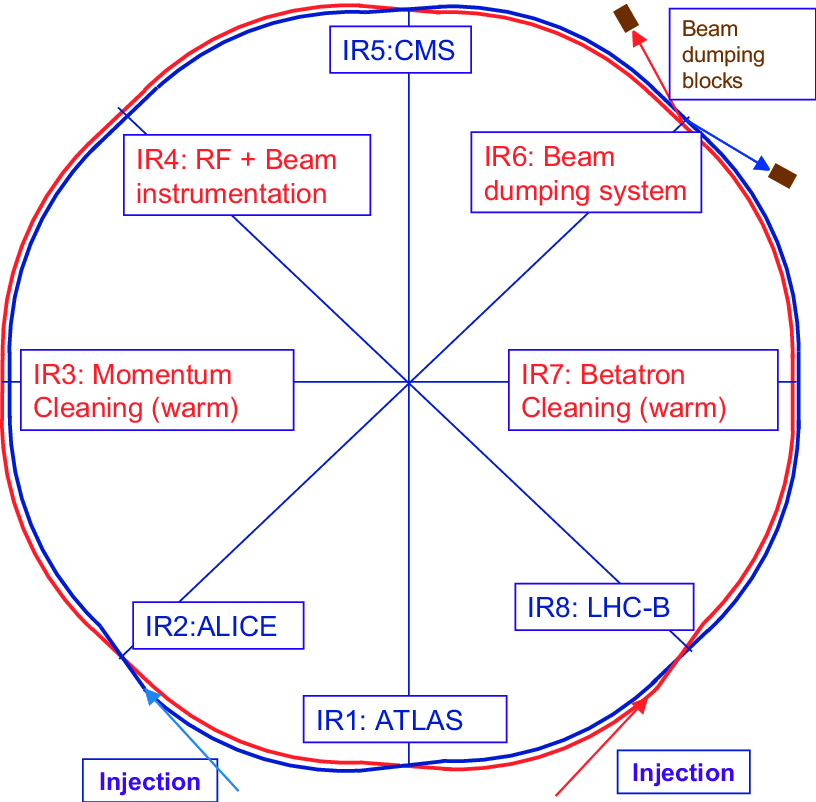
\includegraphics[width=\textwidth,keepaspectratio]{Layout.png}
		\caption[Beam pipes]{LHC beam pipes and crossing points.}
		\label{fig::pipes}
	\end{subfigure}
	\caption{Schematic depiction of the LHC ring.}
	\label{fig::layout}
\end{figure}

     The LHC has inherited its 27 km tunnel from the predecessor, an electron-positron collider called Large Electron-Positron (LEP). However, all the LEP hardware has been replaced to sustain the conditions of the LHC beam. About 2/3 of the LHC circumference length is occupied by the dipole magnets that bend the trajectory of the proton beam to keep it within the pipe. These magnets use superconducting coils that conduct a current of 11080 amperes to produce a magnetic field of 8.3 Tl.\\
     Proton acceleration is maintained by the radio-frequency (RF) cavities (Fig. \ref{fig::rf_cavities}). Besides the acceleration particles the RF cavities are also responsible for beam bunching i.e. separating the beam into a train of separated particle packs, each containing about $10^{11}$ protons. During LHC Run 2 the bunches were separated by 7 meters (25 ns) with a maximum of 2556 circulating bunches.
	\begin{figure}[htbp]
	\begin{subfigure}[t]{0.48\textwidth}
		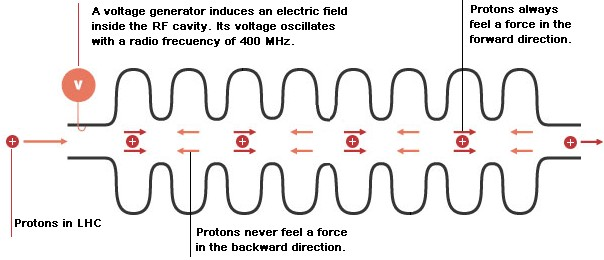
\includegraphics[width=\textwidth,keepaspectratio]{rf_cavities.jpg}
		\caption[RF Cavities]{The RF cavities \cite{rf_cavities}.}
		\label{fig::rf_cavities}
	\end{subfigure}
	\hfill
	\begin{subfigure}[t]{0.48\textwidth}
		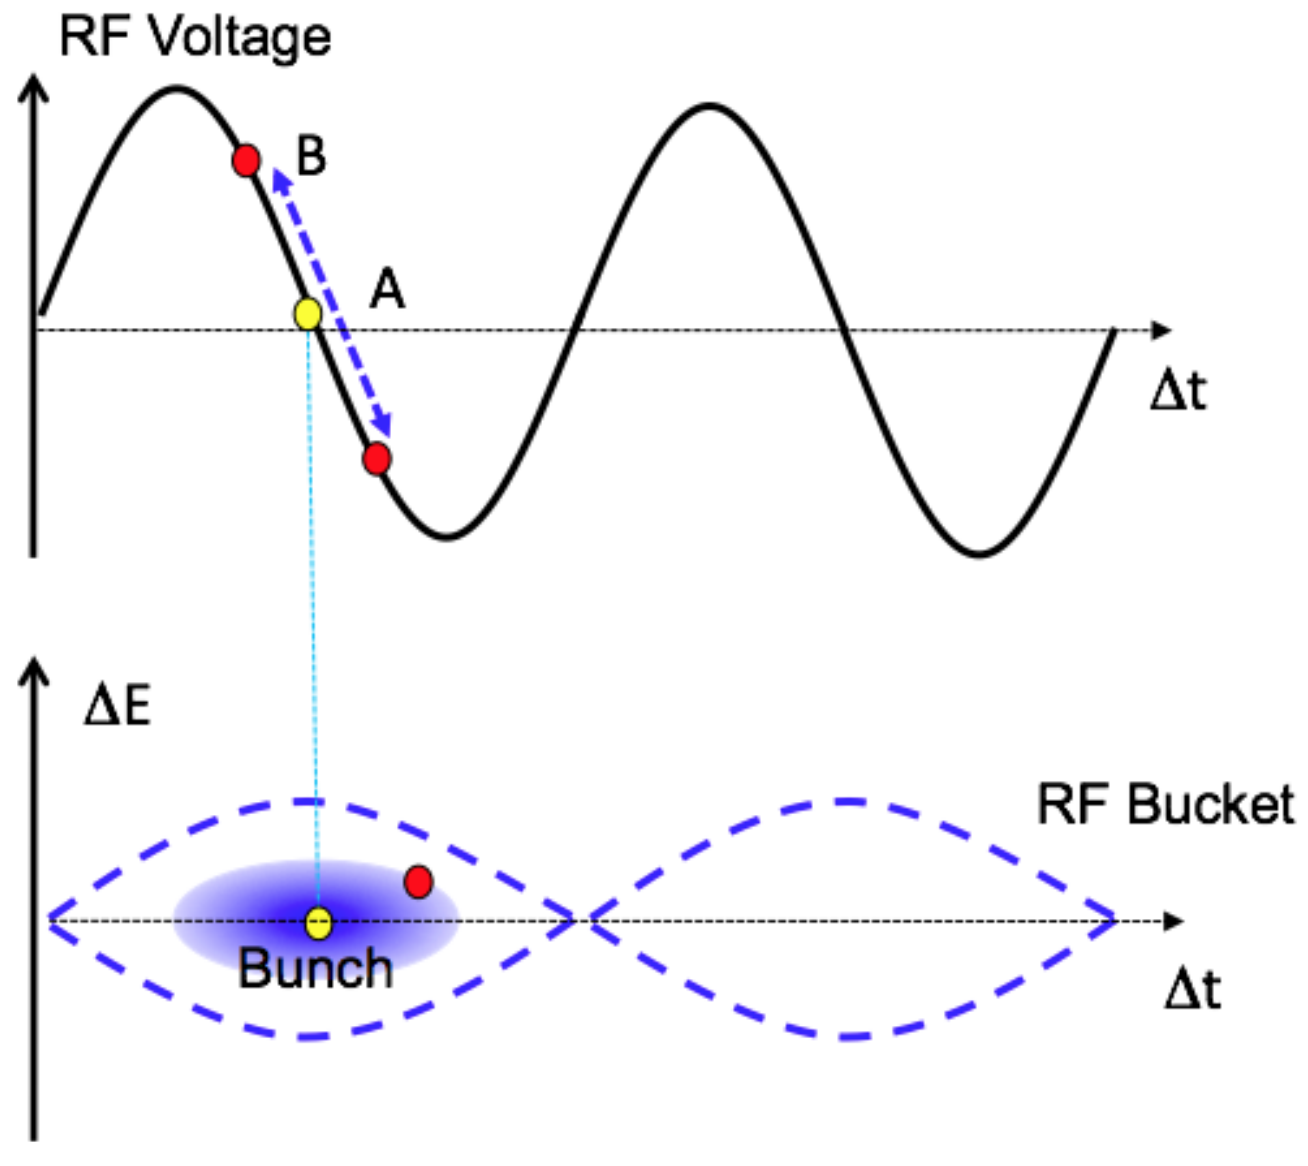
\includegraphics[width=\textwidth,keepaspectratio]{bunch0.png}
		\caption[Beam pipes]{Bunch behaviour at the RF cavities \cite{Wilson:513326}.}
		\label{fig::bunching}
	\end{subfigure}
	\caption{Bunching at RF cavities}
	\label{fig::bunch_at_rf}
\end{figure}
	The LHC has four crossing points, where the two beams are crossed in order to collide protons. Naturally, the particle detectors are installed at these four points. Before getting directed at the crossing point the beams get squeezed to make their cross-section as small as 16 $\mu m^2$ (Fig \ref{fig::2beams}).  	

	\begin{figure}[htbp]
	\begin{subfigure}[t]{0.48\textwidth}
		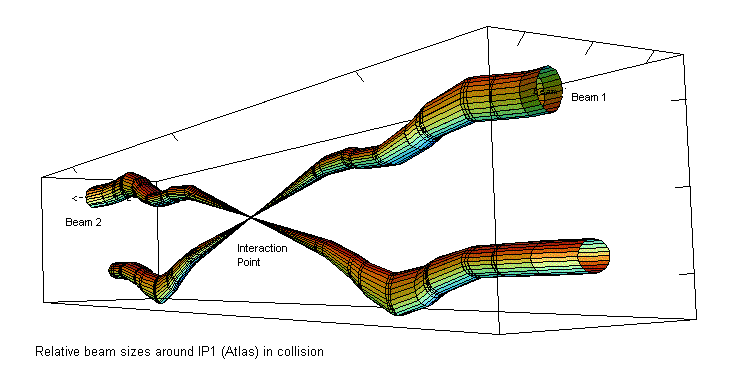
\includegraphics[width=\textwidth,keepaspectratio]{2-beams-IP.png}
		\caption[Two beams]{The two beams getting squeezed at the IP \cite{2beams}.}
		\label{fig::2beams}
	\end{subfigure}
	\hfill
	\begin{subfigure}[t]{0.48\textwidth}
		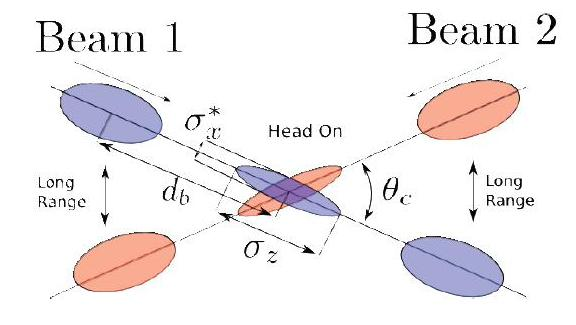
\includegraphics[width=\textwidth,keepaspectratio]{bunch_crossing.jpg}
		\caption[Bunches colliding]{Bunches at the collision point \cite{collisions}.}
		\label{fig::bunches_collision}
	\end{subfigure}
	\caption{Bunch crossing at the LHC.}
	\label{fig::interaction_point}
	\end{figure}
	In order to estimate the number of single proton-proton interactions in the crossing beams a value called instantaneous luminosity (simply called luminosity) is introduced. It is the proportionality factor between the number of events per second $dR/dt$ and the cross-section $\sigma_p$:
	 \begin{equation}
	\nonumber
	\frac{dR}{dt} = \mathcal{L} \cdot \sigma_p.
	\end{equation}
	For the case of head-on collisions the luminosity would equal to \cite{Lumi}:
	\begin{equation}
	\mathcal{L} = \frac{N_1N_2fN_b}{4\Pi \sigma_x \sigma_y},
	\end{equation}
	with $N_1$ and $N_2$ being the intensities of the two colliding beams, $f$ is the revolution frequency, $N_b$ - the number of bunches per beam, $ \sigma_x,\sigma_y$ - the r.m.s. beam widths in the corresponding dimensions, assuming that the bunches in both beams have the same size and Gaussian profiles. \\

	Head-on crossing of the beams would ensure maximal luminosity given the same beams, but on the other hand the measurement would suffer from unwanted beam-to-beam effects. To avoid it the beams at the LHC are crossed at an angle, which is called the crossing angle (see Fig. \ref{fig::bunches_collision}). 
	For the case of head-on collisions the luminosity gets a factor $\mathcal{F} $ \cite{Lumi}:
	\begin{equation}
	\mathcal{L} = \frac{N_1N_2fN_b}{4\Pi \sigma_x \sigma_y} \cdot \mathcal{F},\\
	\end{equation}
	with geometric factor
	\begin{equation}
	\nonumber
	\mathcal{F} = \frac{1}{\sqrt{ 1+\left(  \frac{\sigma_s}{\sigma_x}  \frac{\theta_c}{2} \right) }},
	\end{equation}
	where $\sigma_s$ is the r.m.s. of the bunch length and $\theta_c$ is the crossing angle. Varying the parameters like beam intensity, bunch spacing, beam profile, crossing angle and others becomes a flexible tool for luminosity control. This comes in handy for different physics analysis, as some processes are rare and demand as much luminosity as possible (this is true, for example, for most of the Higgs studies), whereas the others suffer from high pile-up conditions.
	The instantaneous luminosity integrated over a period of time is called the integrated luminosity:
	\begin{equation}
	\mathcal{L}_{int} = \int_0^{T} \mathcal{L}(t) dt,
	\end{equation}
	and is directly related to the number of observed events $\mathcal{L}_{int} \cdot \sigma_p = N_{events}$. A precise measurement of the integrated luminosity is crucial for the LHC results since the uncertainty on it impacts most of the analyses. A comprehensive overview on the luminosity determination at proton colliders can be found here \cite{lumi_witold}. Absolute luminosity measurements at the LHC are performed predominantly using the van-der-Meer (vdM) scan method \cite{vdm1}, \cite{vdm2}. 
	
        \section{Special low pile-up run during LHC Run 2}
        During the Run 2 that lasted from 2015 to 2018 the ATLAS experiment has collected 146.9 $fb^{-1}$ of data under different bunch crossing conditions (see Fig. \ref{fig::run2lumi}). However, the precise measurement of the W boson-related processes demands special conditions. High number of proton-proton collisions per bunch crossing leads to contamination of the final state signal with soft collisions products. This effect, known as pile-up, complicates object reconstruction and results in systematic uncertainties growth. For this reason two special runs with low number of interactions per bunch crossing have been performed by the LHC in 2017 and 2018 at the energies of 5 and 13 TeV. Table \ref{tab:lowmu} contains information on the data collected at ATLAS experiment during the special low pile-up run with $<\mu> \approx 2$.\\
		 \begin{figure}[htpb]
			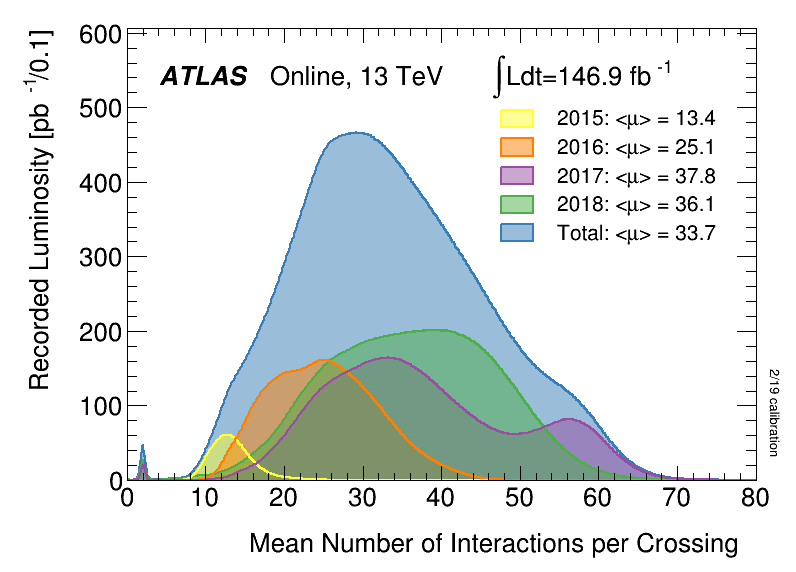
\includegraphics[width=\textwidth,keepaspectratio]{mu_2015_2018.png}
			\caption{ Number of Interactions per bunch crossing in \gls{atlas} Run 2 \cite{run2lumi}. The little bump around $\mu \approx 2$ corresponds to special low pile-up runs.}
			\label{fig::run2lumi}
			\end{figure}
			\begin{table}
			\centering			
			\begin{tabular}{|l|c|c|c|}
			\hline
			\textbf{Collision energy} & \textbf{Year}& \textbf{Integrated luminosity, $pb^{-1}$ }&  Total uncertainty, \%\\
			\hline
			5 TeV  & 2017 & 258& 1.6\\
			13 TeV  & 2017 & 148& 2.1 \\
			13 TeV  & 2018 & 193& 1.5\\
			\hline
			\end{tabular}
			\caption{Energy and luminosity of the special low-mu runs.}
			\label{tab:lowmu}
			\end{table}